\documentclass[aps,pra,notitlepage,amsmath,amssymb,letterpaper,12pt]{revtex4-1}
\usepackage{amsthm}
\usepackage{graphicx}
%  Above uses the Americal Physical Society template for Physical Review A
%  as a reasonable and fully-featured default template
 
%  Below define helpful commands to set up problem environments easily
\newenvironment{problem}[2][Problem]{\begin{trivlist}
\item[\hskip \labelsep {\bfseries #1}\hskip \labelsep {\bfseries #2.}]}{\end{trivlist}}
\newenvironment{solution}{\begin{proof}[Solution]}{\end{proof}}
 
% --------------------------------------------------------------
%                   Document Begins Here
% --------------------------------------------------------------
 
\begin{document}
 
\title{Classwork 01}
\author{Sharon Kim, Kynan Barton, Kristalee Lio}
\affiliation{CS 510, Schmid College of Science and Technology, Chapman University}
\date{\today}

\maketitle
\section{Abstract}
\noindent The derivative is one of the core concepts of calculus. After mastering derivatives, students can apply them to various fields such as statistics, engineering, economics, medicine, etc. This paper provides the first step in understanding derivatives by giving you the definition of a derivative in algebraic and graphical terms. A step by step example is also provided to illustrate how to use the definition of a derivative to calculate the derivative of a function.

\section{The Derivative}

\noindent \textbf{Definition.}
Let \textbf{\textit{y = f(x)}} be a function. The derivative of f is the function whose value at \textbf{\textit{x}} is the limit provided this limit exists.

\begin{align*}
f'(x) &= \lim_{h \to 0} \frac{f(x+h)-f(x)}{h}.
\end{align*}

\noindent If this limit exists for each \textbf{\textit{x}} in an open interval \textbf{\textit{I}}, then we say that \textit{f} is differentiable on \textbf{\textit{I}}.

\bigskip
\noindent \textbf{Example.}
Find the derivative of the following function using the definition of the derivative.
\begin{align*}
f(x) &= 2x^2-16x+35
\end{align*}

\noindent \textbf{Solution.}
Plug this function into the definition of the derivative, and do some algebra. First plug the function into the definition of the derivative. Then multiply everything out. Notice that every term in the numerator that did not have an h in it cancelled out. We can now factor an h out of the numerator which we will cancel against the h in the denominator. After that, we can compute the limit.
\begin{align*}
f'(x) &= \lim_{h \to 0} \frac{f(x+h)-f(x)}{h} \\
&= \lim_{h \to 0} \frac{2(x+h)^2 -16(x+h) +35 -(2x^2-16x+35)}{h} \\
&= \lim_{h \to 0} \frac{2x^2 +4xh +2h^2 -16x -16h +35 -2x^2+16x-35}{h}\\
&= \lim_{h \to 0} \frac{4xh +2h^2 -16h}{h} \\
&= \lim_{h \to 0} \frac{h(4x+2h-16)}{h} \\
&= \lim_{h \to 0} 4x+2h-16 \\
f'(x) &= 4x-16
\end{align*}

\noindent \textbf{Figure.}

\begin{figure}[h!]
 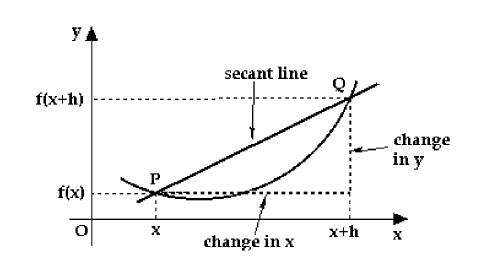
\includegraphics[width=0.6\textwidth]{derivativedefinition.JPG}
  \caption{}
  \label{fig:figlabel}
\end{figure}

\noindent Figure 1 shows a graphical representation of the definition of a derivative. f'(x) represents the slope of f(x) at an arbitrary point in it's domain.

\section{References}
\noindent Lawrence S. Husch. \textit{Husch: Definition of Derivative.} \\ URL: http://archives.math.utk.edu/visual.calculus/2/definition.12/
\\
\\
\noindent Paul Dawkins. \textit{Dawkins: The Definition of the Derivative.} \\ URL: http://tutorial.math.lamar.edu/Classes/CalcI/DefnOfDerivative.aspx
\\
\\
\noindent \textit{Limits and Derivatives} URL: https://learnmathforfree.jimdo.com/calculus/limits-and-derivatives/
\\
\\
\noindent Jeff Cruzan. \textit{Cruzan: The Derivative} URL: http://www.drcruzan.com/TheDerivative.html

\end{document}
